
\chapter{绪论}

\section{数据命名网络}

数据命名网络,Named Data Network\cite{zhang2010named},简称NDN,是未来因特网架构的一部分。
该项目项目旨在开发一个新的互联网架构,可以对互联网目前的基于主机的,点至点的通信体系结构的和地址的弱点进行优化。
该项目研究并加以解决以下问题,以验证NDN作为未来互联网体系结构的技术挑战:
路由的可扩展性,快进,信任模型,网络安全,内容保护和隐私,以及基本的传播理论。
该NDN项目已于2010年9月资助的美国国家科学基金会NSF下的未来互联网体系结构项目的四个项目之一。
不同于现有的IP网络,NDN中不使用端到端的解决方案。


\begin{figure}
\centering
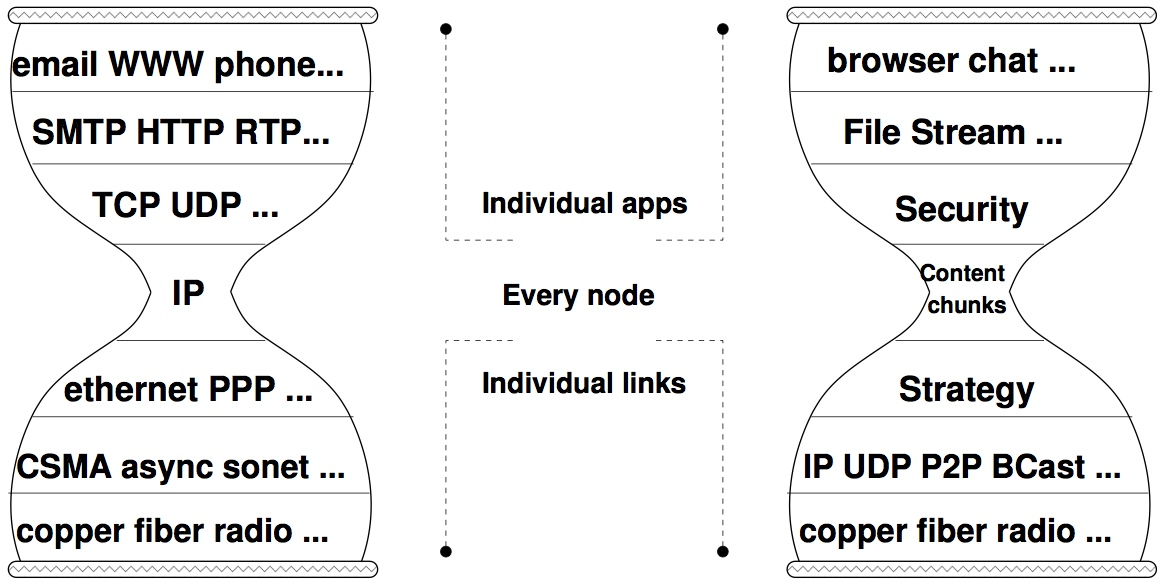
\includegraphics[width=4.5in]{png/ndn_and_ip.jpg}
\caption{NDN和IP的架构比较}
\label{fig:hour_glass}
\end{figure}

\begin{figure}[]
\centering
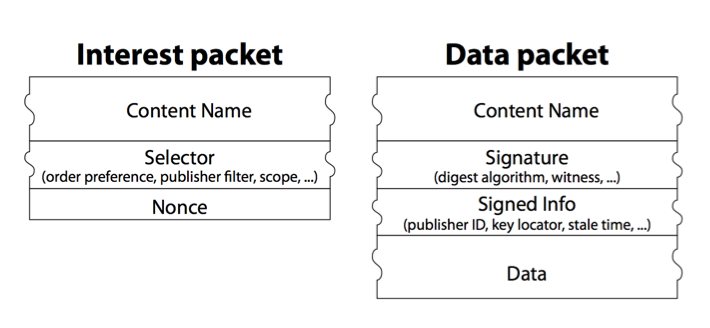
\includegraphics[width=4.5in]{png/ndn_packet.png}
\caption{NDN中得Interest和Data数据包}
\label{fig:interest_data}
\end{figure}

如图\ref{fig:hour_glass}所示,不同于IP的`hour glass'架构,
在NDN通信接收端,数据数据是由消费者驱动的。
在NDN中,存在两种包格式:兴趣包和数据包,如图\ref{fig:interest_data}.
接收数据时,消费者发出一个兴趣分组,它带有用于识别所需要的数据的名称。
例如,消费者可以请求`/ustc/video/a.mpg'。
路由器记得该请求进入的端口,然后在其转发的转发兴趣报列表(FIB )中查找名称。
它是一个基于名字的路由协议。
当兴趣包达到具有所请求的数据的节点时,一个数据包被发送回,
它带有两个名称和内容数据,并带有生产者的签名。
此数据包沿着兴趣分组的反向的路径,回到消费者。
需要注意的是,无论是兴趣包还是数据包,都不携带任何主机或接口地址(如IP地址)。
兴趣包路由到数据是基于兴趣包所包含的报文的名字,数据包产生者根据由兴趣包在每个路由器跳状态信息原路返回。
NDN路由器保持兴趣包和数据一段时间,作为缓存。

\begin{figure}
\centering
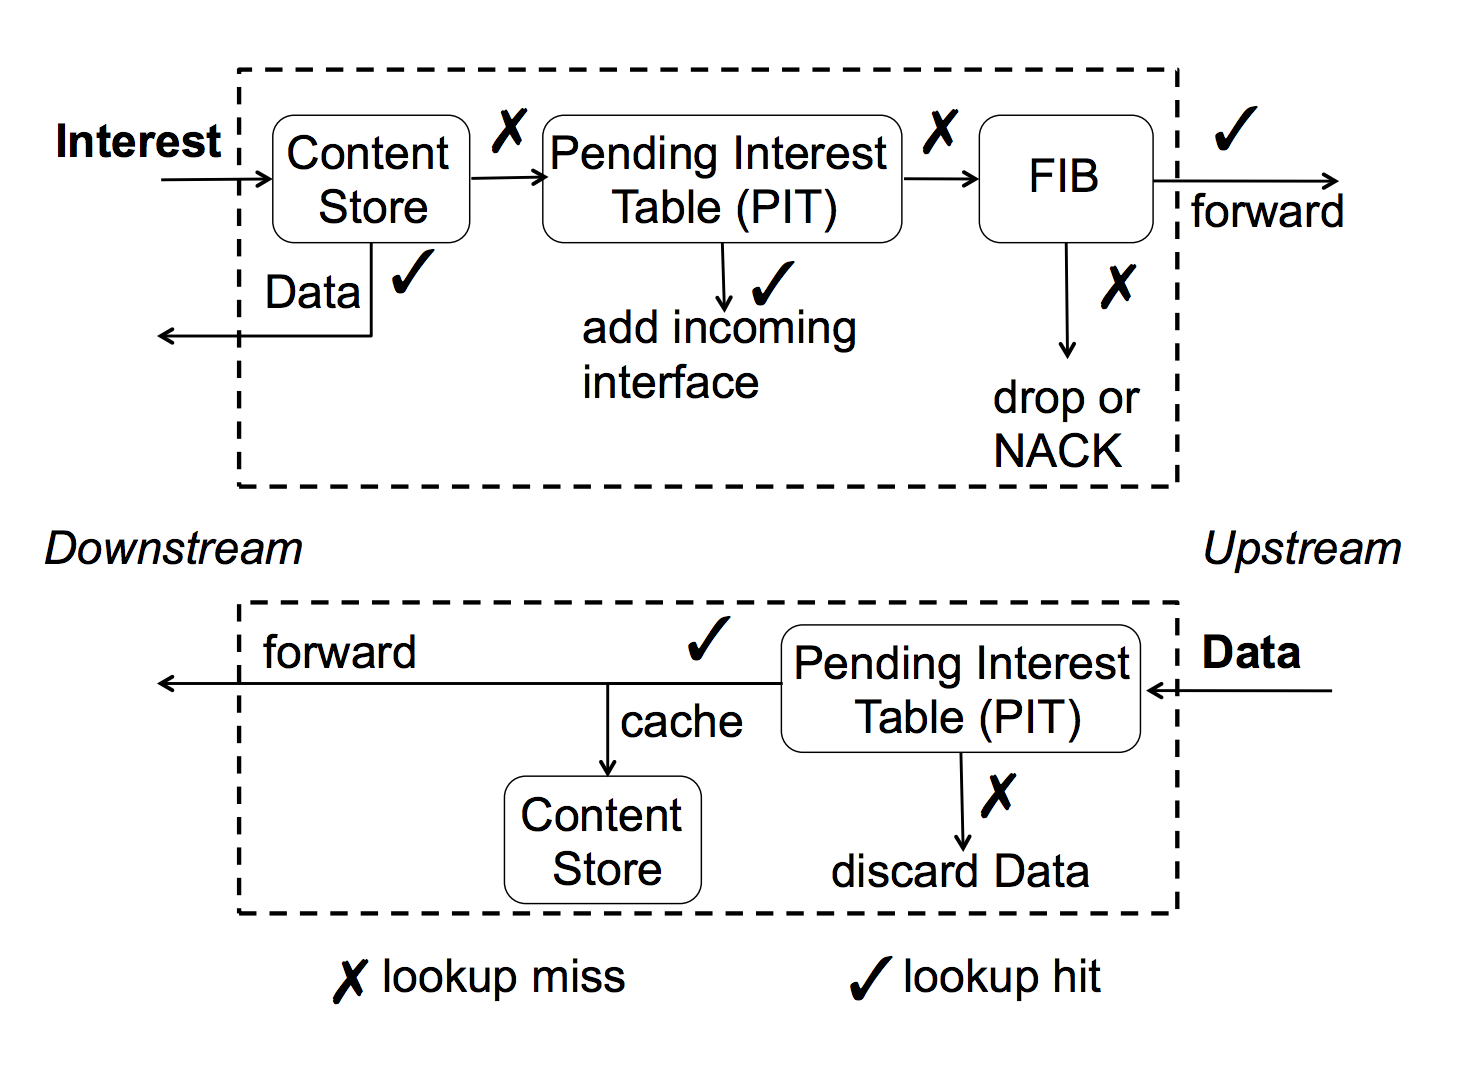
\includegraphics[width=4.5in]{png/interest_data_process.png}
\caption{NDN中处理Interest和Data数据包的流程}
\label{fig:ndn_process}
\end{figure}

在NDN中处理兴趣包时,如图\ref{fig:ndn_process},先查找自己的CS.
如果找到,那么直接返回这个数据,不会将Interest向下一跳传递.
如果没有找到,他会查看自己的PIT表,如果存在,那么在PIT表中添加此端口后丢弃.
这就保证了不会有相同的Interest在同一个链路中传递.
如果PIT中也没有,路由器就会在FIB中查找该名称,以确定向那个端口转发此兴趣包.
如果FIB中也没有,那么返回错误信息.
图\ref{fig:forwarding}描述了这个转发兴趣包的过程.

当多个相同兴趣包所请求的为同一个数据,那么只有第一个对数据源的兴趣包会向上游发送。
该路由器然后将这个转发信息存储在转发兴趣包表( PIT )中 ,
其中每个条目包含兴趣包名和一组从接口,这些接口都是发送该兴趣包来的接口。
当数据包到达时,路由器就会找到与之对应的PIT项和数据转发到所有列出的接口PIT的条目。
路由器然后删除相应的PIT表项,并将其缓存在自己的本地缓存中。
这使用路由器的缓冲存储器,并采用高速缓存替换策略。
数据有请求它的兴趣包的精确相同的路径,但是传输方向相反。
PIT和FIB的结构见图\ref{fig:pit_fib}.

\begin{figure}
\centering
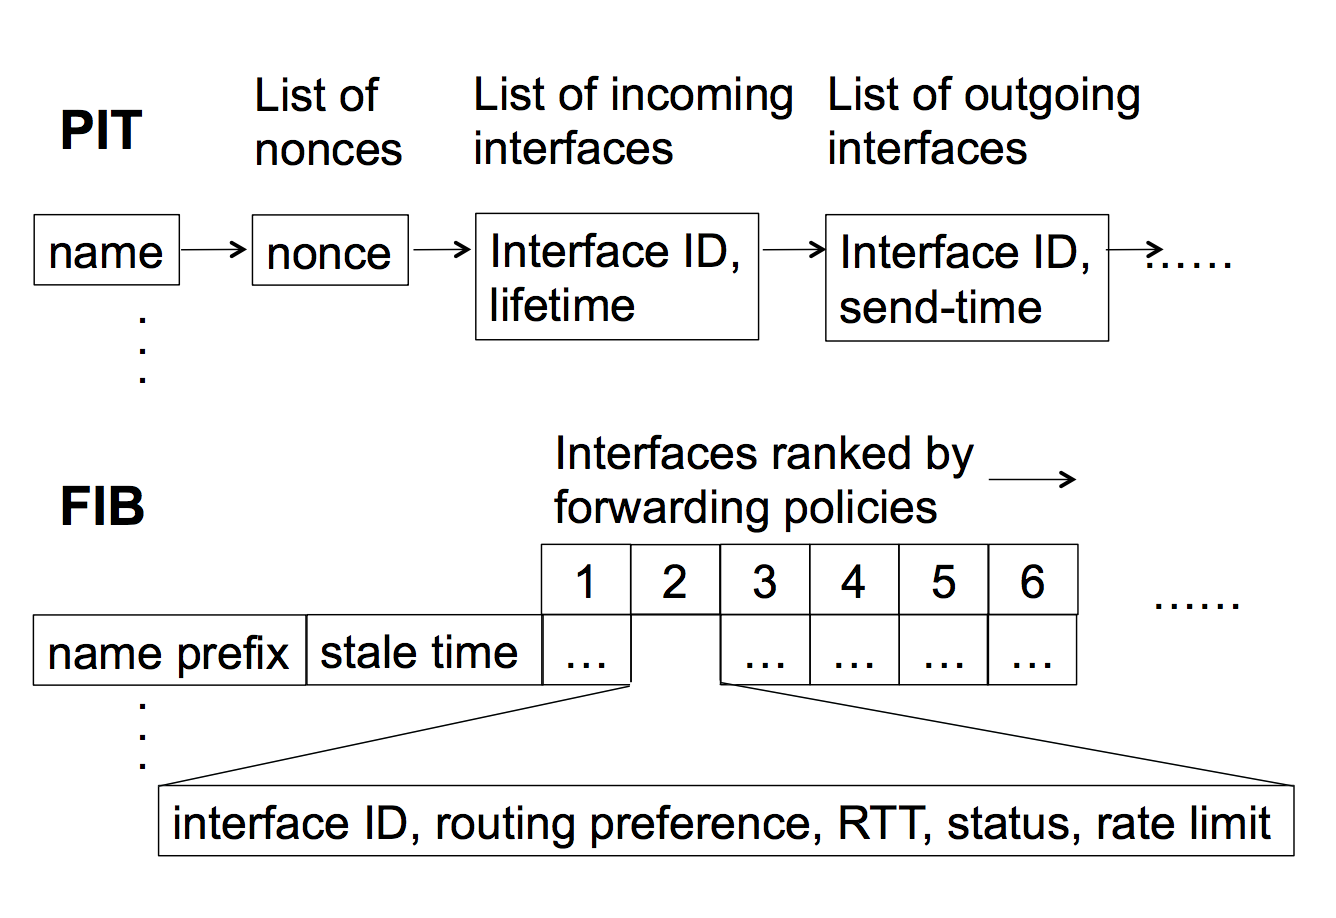
\includegraphics[width=4.5in]{png/pit_fib.png}
\caption{PIT和FIB的结构}
\label{fig:pit_fib}
\end{figure}

\begin{figure}
\centering
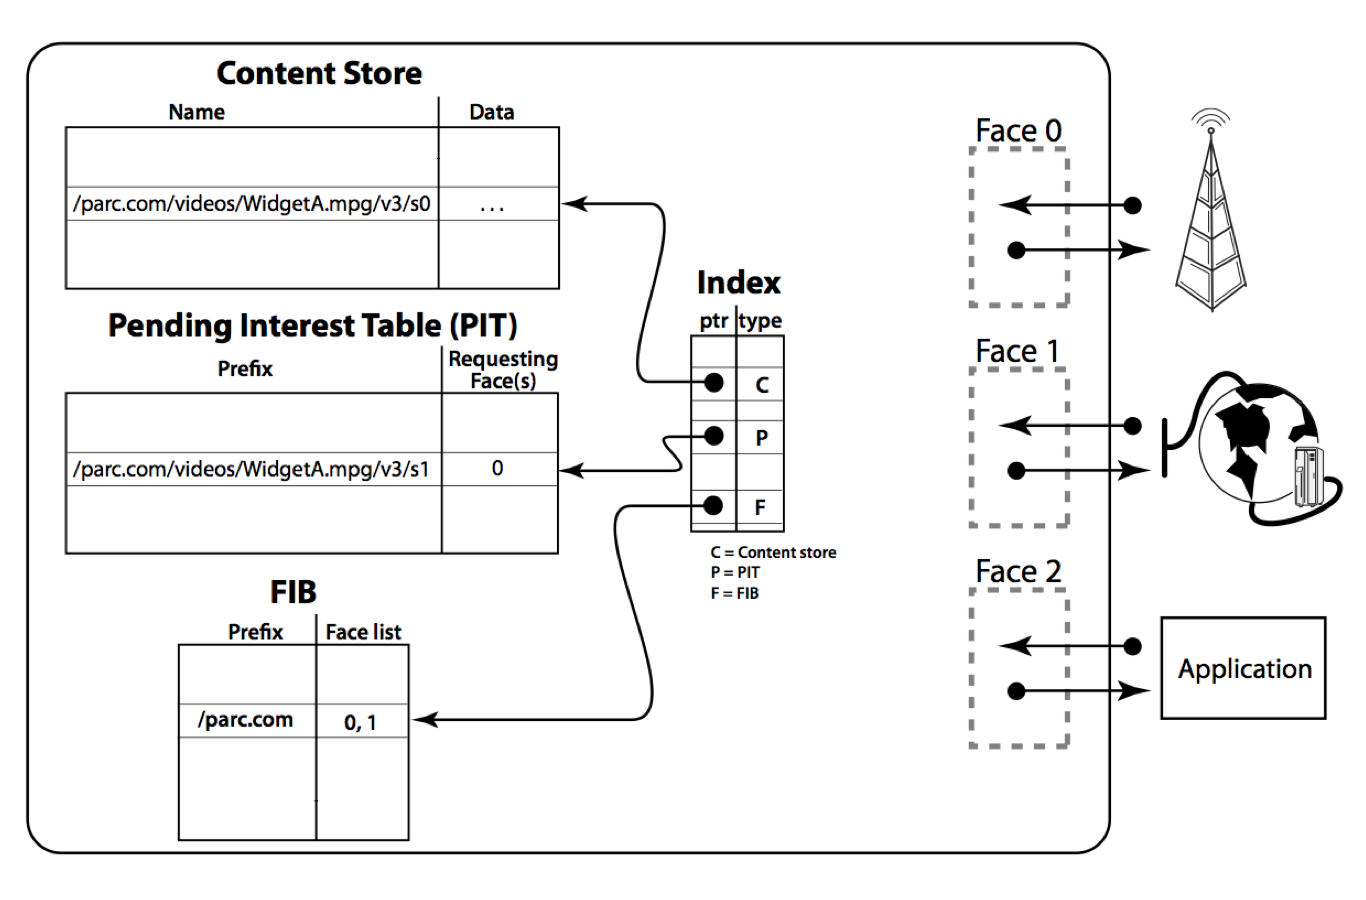
\includegraphics[width=4.5in]{png/forwarding.png}
\caption{一个NDN节点对数据包的转发过程}
\label{fig:forwarding}
\end{figure}


一个数据满足一个兴趣包,在每个跃点,实现逐跳流量平衡。
一个NDN数据包与其是来自何处,或在有可能被转发到的位置是独立的,
因此,路由器可以缓存它来满足未来的潜在需求。
这使NDN自动支持各种功能,而无需额外的基础设施,
包括内容分发(许多用户要求在不同的时间相同的数据),
多播(许多用户请求相同的数据在同一时间),
流动性(用户请求来自不同位置的数据),
并延迟容忍网络(用户有间歇连接)。
例如,考虑一个消费者在移动的车辆中观看流媒体视频。
消费者可以请求一些数据,但然后移动到一个新的本地网络。
虽然数据将在到达旧的位置和被丢弃,但是沿着路径会被缓存。
当消费者重发兴趣包,它可能会从附近的一个缓存中提取数据,使得中断最小。
数据缓存接近消费者提高网络传输性能,并减少对特定数据源的依赖。
这样就能有效避免由于故障或攻击可能导致的失败。

\section{即时多人聊天应用的数据同步问题}

即时多人聊天应用,例如qq,msn等热门应用,
所提供的关键功能是让群体中的每一个人都能向群体中发送消息,接受消息。
不同于两人聊天,多人聊天就涉及到如何让所有人都能收到其他人所发送的消息。
现阶段,此类应用都是运行在现有网络,即IP网络上的。这为其带来了不可避免的弊端。

IP网络被设计成点对点的通信,即通信过程中,整个网络层所知道的是通信源点和目标节点的IP地址。
路由器根据IP地址解析出下一跳的路径,并传递数据包。

在IP网络上,这些应用的同步算法是要有中央服务器的。每个人都和中央服务器建立连接。
中央服务器负责收集每个人的发送的消息,并将这些消息转发给其余所有人。
当一个参与者发送了一条文本信息,此信息会先经过路由到达中央服务器。
中央服务器维护了一个包含所有参与者的列表,
它收到消息后,经过计算处理,然后将此消息转发给需要它的人,以完成功能。

虽然这种办法可行,而且实际上在IP网络上也只能这样运行。
但是这种方法带来了严重的性能问题。

\begin{enumerate}
\item 存在大量的overhead

由于IP是点对点通信,这意味着中央服务器想要将一个消息传递给一个聊天室里的所有成员时,
不得不建立与所有人的TCP连接,并向每一个连接发送一份消息的副本。
如果有两个聊天用户在拓扑上非常近(例如他们连在同一个路由器上,而服务器可能在十跳之外。
这种情况下,需要两个相同的数据包,在这十个路由器上经过,而事实上只需要一个。
在群聊的环境中,用户量更大,更密集,从而造成更加大得多的overhead。
\item 鲁棒性不强

由于所有通信的实现都需要中央服务器的调节,这造成了单点故障。
如果服务器宕机了,或者被不法分子攻击,整个网络中的所有成员均不能正常通讯。
系统也无法自我修复,必须等到服务器维修好后才能重新上线服务。
\end{enumerate}


IP的点对点的通讯模型导致了这些性能瓶颈,
而Named Data Network作为最近发展的一个新的网络架构,为解决这个问题提供了机会。
NDN的优于IP网络模型的根本点在于它不是点对点的模型。
NDN中,所有的资源使用一个独一无二的名字来索引,每个名字对应了一个资源。
资源获取是消费者主导的,也就是说,客户端想要访问一个资源时,
他以此资源的名字发送Interest数据包,并等待接受返回的数据。
由于资源是以名字来定义的,所有请求同一个资源的用户所发送的请求都是一样的:资源的独一无二的名字,
那么NDN中的路由器就会检测到相同的兴趣包,而不会将这个重复的兴趣包向下一跳传递。
当有内容返回时,NDN路由会将这个数据包向所有的端口转发,从而实现多路转发。
除此之外,NDN路由还涉及了缓存机制,当有内容数据包返回时,它会将这个包缓存在自己的内存中。
如果之后有用户请求相同的资源,NDN路由就会发现这个资源已经在自己的缓存中了,于是便可以直接返回给客户端。
这显著的减少了overhead,而且加快了数据包响应时间。

基于NDN的这些特性,它可以为即时多人聊天应用提供很好的架构基础,为解决这个性能瓶颈提供了新的机会。
利用这些特性,以上的问题可以得到较好的解决。
由于NDN的资源是有独特名字的,聊天室里的每一个人想要得到最新消息时,发送的兴趣包是相同的。
NDN路由会过滤掉所有重复的兴趣包,而往下一个路由只发送一份。
当数据返回时,内容包也会只有一份传递回来,并且由路由向各个端口分发数据包。
这样就实现了比传统IP方式小得多的overhead。
另一个方面,由于NDN不关心端点的IP,所有流量都是由Interest包的名字决定的,
因此可以将算法设计成分布式的,当有些节点出现故障,系统仍然可以继续工作,并且可以自我修复。

最近NDN研究人员提出了一种基于此的解决方案,ChronoSync\cite{zhu2013let}。
这个方案是一个完全的分布式的算法,每一个用户都要定期向整个系统广播一个代表他自己当前状态的Interest。
任何人都可以回复这条Interest,只要他认识这个状态,而且他自己的状态更新。
在系统稳定时,每个人都会保留着其他人的Interest,
一旦自己有消息要发送,便立即响应这些Interest,从而将消息发布给团体里的所有人。

ChronoSync为此问题提供了很好的尝试和解决方案,也证明了比IP为基础的算法有明显的优势。
然而,这个算法仍有严重的不足。最大的问题在于,它是一个完全分布的算法,系统没有能力处理特殊情况。
例如,当有两个成员同时发布消息,他们都会响应所保留的别人发来的Interest。
然而,在NDN中,一个Interest只能带回一个数据包,这就必然导致有一个人的消息无法到达。
这样,系统就被分为两个不同阵营,各自有着不同的消息状态,互相无法识别。
更加糟糕的是,当系统里有很多人,出现这种情况的几率将会非常普遍,系统甚至会被分成若干个不同的阵营。
另外,ChronoSync的设计就决定了它无法扩展。每个人需要向全网广播兴趣包,来获取新的消息。
这样这个系统就只能在有限的小范围内使用,如果想在大范围内使用,就必须有分层机制,让复杂度指数递减。

在这种情况下,我们提出了TreeSync来解决此问题。我们的设计目标有以下几点:

\begin{enumerate}
  \item 必须是分布式的。这样才能是系统更健壮,鲁棒性更强。
  \item 有能力处理特殊情况,包括多个并发的消息。
  \item 要能在大范围内进行扩展。
\end{enumerate}

我主要完成的工作有:

\begin{enumerate}
  \item 设计了TreeSync来解决NDN中即时多人聊天应用的信息同步问题。
  \item 在ndnSIM\cite{afanasyev2012ndnsim}中做了仿真。
  \item 与ChronoSync做对比,证明算法的优越性。
\end{enumerate}

接下来各章将会按照如下方式展开。
在第\ref{chapter:relatedwork}章,将会讨论现有的工作,ChronoSync,以及其不足.
第\ref{chapter:design}章,将会详细讨论算法的设计细节。
第\ref{chapter:simu}章叙述在ndnSIM中的仿真情况,并将结果与ChronoSync作对比。
我们将在第\ref{chapter:conclude}章总结全文,展望未来.
